\section{Introduction}
\label{sec:introduction}

Recent years have seen a proliferation in the use of graph processing technologies \cite{Besta2019}. Application areas are wide reaching from healthcare, to social networks and fraud detection \cite{Eifrem2016}. Graph databases model data as a \textit{property graph} \cite{Robinson2015}, vertices represent entities and edges represent the relationships between entities. In addition, properties can be stored on both vertices and edges. In the storage layer, edges are represented by two reciprocal pointers, one stored with each vertex the edge connects. This allows for bi-directional traversal and improved query performance \cite{Robinson2015}. An edge is said to be \emph{reciprocally consistent}, if its two end pointers are mutually reciprocal of each other (details in Section \ref{sec:recipr-cons}).

In practice, graphs can be extremely large, sometimes in the magnitude of 100 billion edges \cite{Sahu2017}, exceeding the storage capacity of a single-node graph database and motivating the need for distributed graph databases. A common distributed graph database design pattern is to first partition graph data over several machines in a cluster; resulting in a number of \emph{distributed edges}, an edge's reciprocal pointers reside in different partitions. Recent work \cite{Ezhilchelvan2018} and \cite{Webber2019} highlighted that violations of reciprocal consistency in distributed edges introduce corruption into the database. Moreover, due to the \emph{Scale-Free} \cite{ScaleFree} property exhibited by many real world graphs, this corruption can propagate through the database at alarmingly rates.

When, for example, a BASE database \cite{Pritchett2008} is adapted with a graph processing layer, then violations of reciprocal consistency will occur if that adaptation provides no concurrency control for operations that span partitions in order to offer higher performance. This paper proposes a simple concurrency control protocol, called \tDelta protocol, that does not impede performance adversely. That is because the protocol is exclusively designed for one purpose only: reciprocal consistency in distributed edges.  Its design leverages the fact that the updating of end pointers of a given distributed edge immediately follow each other and the small interval between them is the window for possible conflicts between concurrent updates. The protocol ensures that any two updates on any given end pointer of any given edge are at least $\Delta$ time apart by aborting any write attempt that is within . It ensures reciprocal consistency when $\Delta$ is chosen to be larger than the length of the conflict window.

The paper is organized as follows: Section \ref{sec:recipr-cons} presents reciprocal consistency, Sections \ref{sec:distr-graph-datab}-\ref{sec:db-corruption} discuss the architecture of distributed graph databases and describes how corruption occurs. Section \ref{sec:tdelta-protocol} outlines the \tDelta protocol. Sections \ref{sec:modeling}-\ref{sec:evaluation} presents the model used to evaluate protocol performance.

\begin{figure}[ht!]
  \centering
  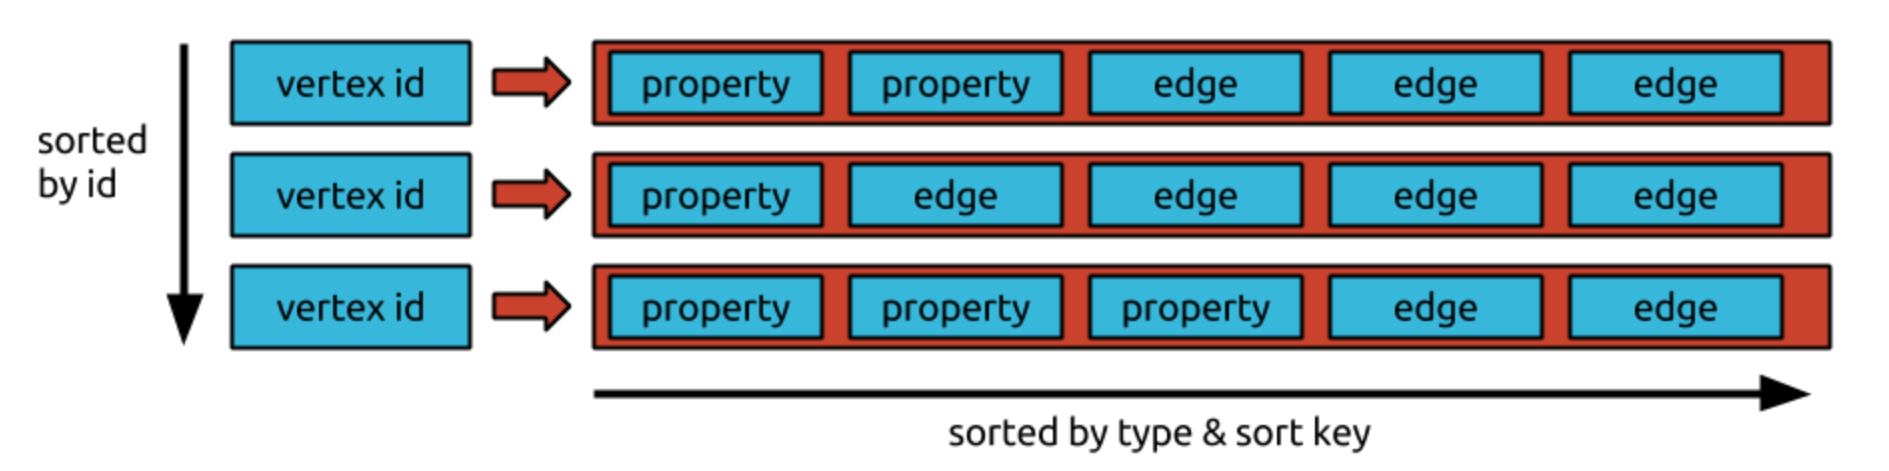
\includegraphics[width=\linewidth]{./figures/janusgraph-adj-list}
  \caption{Database records representing vertices, containing properties and a sequence of edges that comprise the adjacency list of a vertex \cite{janusgraph}.}
  \label{adj-list}
\end{figure}